% Created 2024-08-08 Thu 17:23
% Intended LaTeX compiler: lualatex
\documentclass{beamer}
\usetheme{default}
\date{\today}
\title{}
\hypersetup{
 pdfauthor={},
 pdftitle={},
 pdfkeywords={},
 pdfsubject={},
 pdfcreator={Emacs 29.4 (Org mode 9.6.15)}, 
 pdflang={English}}
\begin{document}

\begin{frame}{Sumário}
\tableofcontents
\end{frame}

\begin{frame}[label={sec:org247bcb0}]{Introdução}
\begin{block}{Breve Histórico}
\begin{mybox}{Precusores}


\begin{itemize}
\item 1807 - Jöns J. Berzelius – Teoria da Força Vital.
\item 1828 – primeiro composto orgânico sintetizado em laboratório – Uréia
\end{itemize}
\begin{center}
\schemestart
\chemname{\chemfig{NH_4CNO}}{Cianato \\ de amônio}
\arrow{->[\(\Delta\)][]}
\chemname{\chemfig{O=C([:30]-NH_2)([:330]-NH_2)}}{Ureia}
\schemestop
\end{center}

\begin{itemize}
\item Tudo que tem “vida” possui compostos orgânicos,mas nem todos compostos orgânicos possuem vida.
\item 1851 à 1861 – Friederich A. Kekulé
\begin{itemize}
\item Formulou três postulados que vigoram até hoje.
\end{itemize}
\end{itemize}
\end{mybox}
\end{block}


\begin{block}{Postulados de Kekulé}
\begin{myrule}{Postulado 1}

\begin{itemize}
\item Os átomos de carbono são tetravalentes.
\end{itemize}
\begin{center}
\chemfig{H-C([:90]-H)([:-90]-H)-C([:90]-H)([:-90]-H)-H}
\end{center}

\begin{itemize}
\item Ligações Covalentes
\end{itemize}

\begin{center}
\chemfig{H-C~C-C([:90]-H)([:-90]-H)-H}
\end{center}

\end{myrule}
\end{block}


\begin{block}{Ligações Múltiplas}

\begin{talltblr}[
	 theme= fancy,
	 caption={Composição do Petróleo},
	 ]{
	 colspec = {Xcc}, colsep = 2mm, hlines = {2pt, white},
	 %row{odd} = {brown8}, row{even} = {gray8},
	 row{1} = {2em,azure2,fg=white,font=\bfseries\sffamily},
	 }
	 \hline
	 Tipo de Ligação & Exemplo & Estrutura de Lewis\\[0pt]
	 \hline
	 Ligação \alert{dupla} entre dois átomos de carbono & \chemfig{C([:210]-)([:150]-)=C([:30]-)([:330]-)} & \chlewis{0:120.240.}{C}  \chlewis{180:60.290.}{C}\\
	 \hline
	 Ligação \alert{dupla} entre um átomo de oxigênio e carbono & \chemfig{C([:210]-)([:150]-)=O} & \chlewis{0:120.240.}{C} \chlewis{180:90:0:}{O}\\
	 \hline
	  Ligação \alert{tripla} entre dois átomos de carbono & \chemfig{-C~C-} & \chlewis{0:50.180.}{C} \chlewis{180:130.0.}{C}\\
	 \hline
	 Ligação \alert{tripla} entre um carbono e nitrogênio & \chemfig{-C~N } & \chlewis{0:50.180.}{C} \chlewis{180:130.0:}{N}\\[0pt]
	 \hline
 \end{talltblr}
\end{block}


\begin{block}{Postulados de Kekulé}
\begin{myrule}{Postulado 2}


\begin{itemize}
\item As quatro valências do carbono são equivalentes.
\end{itemize}

\begin{figure}[htbp]
\centering
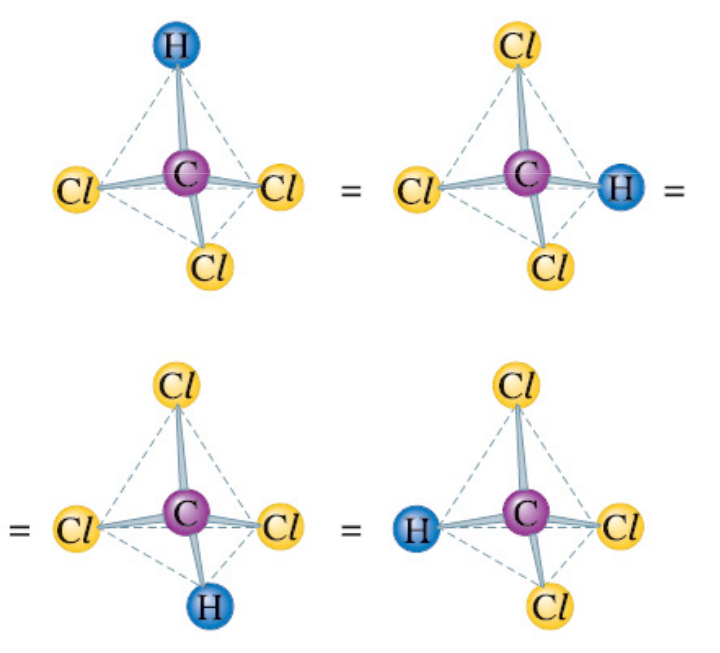
\includegraphics[width=0.45\textwidth]{../Fundamentos/cloroformio.png}
\caption{\label{fig:orge5e92a0}Clorofórmio}
\end{figure}

\end{myrule}
\end{block}


\begin{block}{Postulados de Kekulé}
\begin{myrule}{3º Postulado}

\begin{itemize}
\item O carbono possui a capacidade \alert{ÚNICA} de formas cadeias.
\end{itemize}



\begin{tblr}{cc}
\chemfig{H-C([:90]-H)([:-90]-H)-C([:-90]-H)=C([:-90]-H)-C([:90]-H)([:-90]-H)-H}& 
\chemfig{C*6((-H)=C(-H)-C(-H)=C(-H)-C(-H)=C(-H)-)} \\
\chemfig{H-[:210]C(-[:120]H)-[:300]C(-[:20]C(-[:320]H)(-[:20]H)-[:80]H)(-[:300]H)-[:210]C(-[:300]H)(-[:210]H)-[:120]C(-[:30]\phantom{C})(-[:210]H)-[:120]H} & 
%\qquad \qquad \chemfig{>[:330](-[:330]-[:30]-[:330])(<:[:60])-[:210](-[:270])-[:150](-[:90])-[:210]-[:150]}
\chemfig{H-[:276]C(-[:12]H)-[:180]C(-[:84]H)(-[:168]H)-[:252]C(-[:156]H)(-[:240]H)-[:324]C(-[:228]H)(-[:312]H)-[:36]C(-[:108]\phantom{C})(-[:24]H)-[:300]H}\\
\end{tblr}

\end{myrule}
\end{block}
\end{frame}


\begin{frame}[label={sec:org341e25b}]{Carbonos}
\begin{block}{Classificação dos carbonos}
\begin{center}
\begin{tabular}{|c|c|}
\hline
\cellcolor{green!20} {\bfseries Carbono}  & \cellcolor{green!20} {\bfseries Definição} \\[0pt]
\hline
Primário & ligado diretamente, \alert{no máximo}, a \alert{1} outro carbono\\[0pt]
\hline
Secundário & ligado diretamente a \alert{2} outros carbonos\\[0pt]
\hline
Terciário & ligado diretamente  a \alert{3} outros carbonos\\[0pt]
\hline
Quartenário & ligado diretamente a \alert{4} outros carbonos\\[0pt]
\hline
\end{tabular}
\end{center}



\begin{columns}
\begin{column}{0.7\textwidth}
\chemfig[scale=2.5]{H_3@{A}C-@{L}C([:-90]-@{B}CH_3)=@{F}CH-@{G}C~@{H}C-@{N}C([:90]-@{D}CH_3)([:-90]-@{K}CH_2(-[:270,,1,1]@{M}CH-[:300,,1,1]@{J}CH_2-[:180,,1,2]H_2@{I}C(-[:60,,2]\phantom{C})))-@{E}CH_3}
\chemmove{
\node[bal,fit=(A)]{};
\node[bal,fit=(B)]{};
\node[bal,fit=(D)]{};
\node[bal,fit=(E)]{};
\node[rect,fit=(F)]{};
\node[rect,fit=(G)]{};
\node[rect,fit=(H)]{};
\node[rect,fit=(I)]{};
\node[rect,fit=(J)]{};
\node[rect,fit=(K)]{};
\node[bal2,fit=(L)]{};
\node[bal2,fit=(M)]{};
\node[bal3,fit=(N)]{};
}
\end{column}
\begin{column}{0.3\textwidth}  %%<--- here
      carbonos \chemfig{@{A}C} = primários\\
      carbonos \chemfig{@{B}C} = secundários\\
      carbonos \chemfig{@{D}C} = terciários\\
      carbonos \chemfig{@{E}C} = quartenários
     \chemmove{
      \node[bal,fit=(A)]{};
      \node[rect,fit=(B)]{};
      \node[bal2,fit=(D)]{};
      \node[bal3,fit=(E)]{};
      }
\end{column}
\end{columns}
\end{block}
\end{frame}


\begin{frame}[label={sec:orgb730017}]{Cadeias}
\begin{block}{Cadeias Carbônicas}
\begin{myrule}{Heteroátomo}

\begin{itemize}
\item Estrutura formada por todos os átomos de carbono e os heteroátomos.
\item Heteroátomo é um átomo diferente do carbono e do hidrogênio  posicionado
entre  dois  carbonos  na cadeia.
\end{itemize}

\chemname{\chemfig{CH_3-CH_2-{\color{red}O}-CH_2-CH_3}}{Oxigênio é heteroátomo}

\vspace{.5cm}\chemname{\chemfig{CH_3-CH_2-CH_2-CH_2-{\color{red}O}H}}{Oxigênio NÃO é heteroátomo}

\end{myrule}
\end{block}




\begin{block}{Classificação das Cadeias Carbônicas}
\begin{myrule}{Cadeia aberta}

\begin{itemize}
\item \emph{Cadeia aberta ou aciclíca:} Os átomos de carbono se ligam entre si de modo a terem os extremos livres
\end{itemize}

\begin{center}
\schemestart
\chemfig{-@{b}{C}([:90]-)([:-90]-)-C([:90]-)([:-90]-)-C([:90]-)([:-90]-)-@{a}{C}([:90]-)([:-90]-)-}
\schemestop 
\chemmove{\draw[<-,red,shorten <=3.5pt] (b) (-0.5,-0.2)--++(1,-0.4) node[below] {extremo livre} ;
\draw[->,red,shorten <=3.5pt] (a) (-4.7,-.9)--++(1.5,0.7) node[anchor=35,inner sep=23] {extremo livre} ;
}
\vspace{1cm}
%
\end{center}

\end{myrule}


\begin{myrule}{Cadeia Fechada}

\begin{itemize}
\item \emph{Cadeia fechada ou ciclíca:} Os átomos de carbono se ligam entre si de modo a formarem um ciclo.
\end{itemize}

\begin{center}
\chemfig{-[:90]C(-[:180])-C(-[:270])(-)-[:90]C(-)(-[:90])-[:180]C(-[:270]\phantom{C})(-[:90])-[:180]}
\end{center}

\end{myrule}


\begin{myrule}{Cadeia Mista}

\begin{itemize}
\item Os atomos se ligam formando um ciclo e tem as extremidades livres.
\end{itemize}
\begin{center}
\chemfig{-[:90]C(-[:180])-C(-[:90]C(-)(-[:90])-[:180]C(-[:90])(-[:180])-[:270]\phantom{C})(-[:270])-C(-[:270])(-[:90,,,1])-C(-[:90])(-[:270])-C(-[:90])(-)-[:270]}
\end{center}

\end{myrule}
\end{block}
\end{frame}


\begin{frame}[label={sec:orgf1b6157}]{Cadeias Abertas}
\begin{block}{Cadeias Abertas}
\begin{tblr}[
		theme= fancy,
		caption={Classificação das Cadeias},
		]{
			colspec = {XX}, colsep = 2mm, hlines = {2pt, white},
			%row{odd} = {brown8}, row{even} = {gray8},
			row{1} = {2em,azure2,fg=white,font=\bfseries\sffamily},
		}

	Cadeia aberta Normal   &  Cadeia Aberta Ramificada \\
%
		Carbonos, primários, secundários & Ao menos um carbono terciário ou quartenário\\
	\chemfig{-(!\nobond\chemabove[1ex]{}{\color{blue}1})C([:-90]-)([:90]-)-(!\nobond\chemabove[1ex]{}{\color{blue}2})C([:-90]-)([:90]-)-C(!\nobond\chemabove[1ex]{}{\color{blue}3})([:90]-)([:-90]-)-} &  \chemfig{-(!\nobond\chemabove[1ex]{}{\color{blue}1})C([:-90]-)([:90]-)-(!\nobond\chemabove[1ex]{}{\color{blue}2})C([:-90]-C(!\nobond\chemabove[1ex]{}{\color{blue}\hspace{.2cm}\vspace{.7cm}4})([:0]-)([:180]-)-)([:90]-)-C(!\nobond\chemabove[1ex]{}{\color{blue}3})([:90]-)([:-90]-)-}\\
		Carbono 1: primário & \\
		Carbono 2: secundário & Carbono 2: terciário\\
		Carbono 3: primário & Carbonos 1, 3 e 4: primários\\
		\hline
	\end{tblr}




\begin{tblr}[
		theme= fancy,
		caption={Classificação das Cadeias},
		]{
			colspec = {cc}, colsep = 2mm, hlines = {2pt, white},
			%row{odd} = {brown8}, row{even} = {gray8},
			row{1} = {2em,azure2,fg=white,font=\bfseries\sffamily},
		}
  Cadeia aberta homogênea   &  Cadeia aberta heterogênea \\
Apresentam somentes átomos de carbono & Ao menos um átomo heteroátomos\\
 \chemfig{-C([:-90]-)([:90]-)-C([:90]-)=C([:90]-)([:-90]-)-} &  \chemfig{-C([:90]-)([:-90]-)-C([:90]-)([:-90]-)-{\color{blue}O}-C([:90]-)([:-90]-)-} \\
 \chemfig{-C([:90]-)([:-90]-)-C([:90]-)([:-90]-C([:180]-)([:0]-)-)-C([:90]-)([:-90]-)-{\color{red} O}-}  &  \chemfig{-C([:90]-)([:-90]-)-C([:-90]-C([:180]-)([:0]-)-)={\color{blue}N}-C([:90]-)([:-90]-)-C([:90]-)([:-90]-)-} \\
Este \emph{oxigênio} não é heteroátomo & \\
\hline
\end{tblr}



\begin{tblr}[
		theme= fancy,
		caption={Classificação das Cadeias},
		]{
			colspec = {XX}, colsep = 2mm, hlines = {2pt, white},
			%row{odd} = {brown8}, row{even} = {gray8},
			row{1} = {2em,azure2,fg=white,font=\bfseries\sffamily},
		}
Cadeia aberta saturada   &  Cadeia aberta insaturada \\
Apresentam somentes átomos de carbono apresentam ligações simples & Apresenta ao menos dois átomos de  carbono ligados pela dupla ou tripla ligação\\
 \chemfig{-C([:-90]-)([:90]-)-C([:90]-)([:-90]-)-C([:90]-)([:-90]-)-} &  \chemfig{-C([:90]-)([:-90]-)-{\color{blue}C}([:-90]-)={\color{blue}C}([:-90]-)-} \\
 \chemfig{-C([:90]-)([:-90]-)-C([:90]-)([:-90]-C([:180]-)([:0]-)-)-C([:90]-)([:-90]-)-{\color{red} O}-}  &  \chemfig{-C([:90]-)([:-90]-)-C-{\color{blue}C}(~[4,,,,blue]{\color{blue}C})-C([:90]-)([:-90]-)-C([:90]-)([:-90]-)-} \\
O átomo de carbono que apresenta ligação simples é chamado de \emph{carbono saturado}. & A átomo que apresenta ligação dupla ou tripla é chamado de \emph{carbono insaturado.}\\
\hline
\end{tblr}
\end{block}
\end{frame}


\begin{frame}[label={sec:org503ebc9}]{Cadeias Fechadas}
\begin{block}{Cadeias Fechadas}
	{\small
\begin{tblr}[
		theme= fancy,
		caption={Classificação das Cadeias Fechadas},
		]{
			colspec = {XX}, colsep = 2mm, hlines = {2pt, white},
			%row{odd} = {brown8}, row{even} = {gray8},
			row{1} = {2em,azure2,fg=white,font=\bfseries\sffamily},
		}
 Cadeia fechada aromática   &  Cadeia fechada alicíclica \\
Cadeia cíclica formada por 6 átomos de carbono alternados em simples e duplas ligação & Cadeia cíclica que não constitui anel benzênico\\
 \chemfig{C*6((-)=C(-)-C(-)=C(-)-C(-)=C(-)-)} & \chemfig{C*6((-)=C(-)-C(-)-C(-)-C(-)=C(-)-)} \\ 
 \chemfig{C*6((-)-C(-)=C(-)-C(-)=C(-)-C(-)=)}   &    \chemfig{-[:90]C(-[:180])-C(-[:270])(-)-[:90]C(-)(-[:90])-[:180]C(-[:270]\phantom{C})(-[:90])-[:180]} \\
Esses ciclos recebem o nome de \emph{benzeno} & \\
\hline
\end{tblr}
}



	{ \setchemfig{atom style={scale=0.5}}
	\begin{tblr}[
		theme= fancy,
		caption={Classificação das Cadeias Fechadas},
		]{
			colspec = {XX}, colsep = 2mm, hlines = {2pt, white},
			%row{odd} = {brown8}, row{even} = {gray8},
			row{1} = {2em,azure2,fg=white,font=\bfseries\sffamily},
		}
		Cadeia aromática mononuclear   &  Cadeia aromática polinuclear \\
		%\hline 
		Cadeia aromática com apenas um núcleo benzênico & Cadeia aromática com dois ou mais núcleos benzênicos\\ 
		\chemfig{C*6((-)=C(-)-C(-)=C(-)-C(-)=C(-)-)}   &  \chemname{\chemfig{C*6((-)=C(-)-C(*6(-C(-)=C(-)-C(-)=C(-)-C))=C-C(-)=C(-)-)}}{Cadeia aromática\\ polinuclear condensada} \\ & \chemname{\chemfig{C*6((-)=C(-)-C(-)=C(-C*6((-)=C(-)-C(-)=C(-)-C(-)=C(-)-))-C(-)=C(-)-)}}{Cadeia aromática \\ polinuclear isolada}\\
		%Esses clicos recebem o nome de \emph{benzeno} & \\[0pt]
		\hline
	\end{tblr}
}



\begin{tblr}
	[
	theme= fancy,
	caption={Classificação das Cadeias Fechadas},
	]{
		colspec = {Xm{8cm}}, colsep = 2mm, hlines = {2pt, white},
		%row{odd} = {brown8}, row{even} = {gray8},
		row{1} = {2em,azure2,fg=white,font=\bfseries\sffamily},
	}
	Cadeia alicíclica homocíclica   &  Cadeia alicíclica heterocíclica \\
	\hline
	Cadeia cíclica alicíclica formada apenas por átomos de carbono & Cadeia cíclica alicíclica que apresenta heteroátomo\\
	\chemfig{-[:90]C(-[:180])-C(-[:270])(-)-[:90]C(-)(-[:90])-[:180]C(-[:270]\phantom{C})(-[:90])-[:180]} & \chemfig{-[:18]C=_[:72]C([:126]-)-C(-[:54,,,1])=_[:288]C([:342]-)-[:216]C(-[:144]\phantom{C})([:207]-)-[:333]}\\ \chemfig{-[:90]C(-[:180])-O([:270])-[:90]C(-)(-[:90])-[:180]C(-[:270]\phantom{C})(-[:90])-[:180]} & \chemfig{-[:18]C=_[:72]C([:126]-)-C(-[:54,,,1])=_[:288]N([:342])-[:216]C(-[:144]\phantom{C})([:207]-)-[:333]}\\
	& \\
	\hline
\end{tblr}


%\pagebreak 
 %\setchemfig{atom style={scale=0.7}}
	\begin{tblr}[
		theme= fancy,
		caption={Classificação das Cadeias Fechadas},
		]{
			colspec = {cX}, colsep = 2mm, hlines = {2pt, white},
			rowspec={QQ},
			%row{odd} = {brown8}, row{even} = {gray8},
			row{1} = {2em,azure2,fg=white,font=\bfseries\sffamily},
		}
%		\hline
Cadeia alicíclica saturada & Cadeia alicíclica insaturada\\
Cadeia cíclica alicíclica formada apenas por ligações simples & Cadeia cíclica alicíclica formada apenas por ligações duplas ou triplas\\
\chemfig{-[:18,,2]C(-[:261])-[:72]C(-[:126])(-[:73])-C(-[:54])(-[:97])-[:288]C(-[:342])(-[:299])-[:216]O(-[:144]\phantom{C})} &  \chemfig{-[:18]C=_[:72]C([:126]-)-C(-[:54,,,1])=_[:288]C([:342]-)-[:216]C(-[:144]\phantom{C})([:207]-)-[:333]} %\chemfig{H_3C-[:18,,2]\mcfbelow{C}{H}-[:72]C~C-[:288]\mcfbelow{C}{H}(-[:342,,,1]CH_3)-[:216]C(-[:144]\phantom{C})(-[:207,,,2]H_3C)-[:333,,,1]CH_3} \\ 		\hline
	\end{tblr}
\end{block}
\end{frame}


\begin{frame}[label={sec:orgaa6c72b}]{Exercícios}
\begin{block}{Exemplo 1}
\begin{question}
(\alert{UFAM-PSC}) O pau-rosa, típico da região amazônica, é uma rica fonte natural do óleo essencial conhecido por linalol, o qual também pode ser isolado do óleo de alfazema. Esse óleo apresenta a seguinte fórmula estrutural:

\chemfig{H_3C-C([:-90]-CH_3)=CH-CH_2-CH_2-C([:-90]-CH_3)([:90]-OH)-CH=CH2}
Sua cadeia carbônica deve ser classificada como:

\begin{choice}(2)
\choice acíclica, ramificada, saturada e heterogênea.
\choice acíclica, normal, insaturada e homogênea.
\choice alicíclica, ramificada, insaturada e homogênea.
\choice acíclica, ramificada, insaturada e homogênea.
\choice alicíclica, normal, saturada e heterogênea.
\end{choice}
\end{question}
\end{block}

\begin{block}{}
\begin{answer}[print=true]
Alternativa \alert{d}.

\begin{itemize}
\item É acíclica, ou seja, possui cadeia aberta, com extremidades livres, sem nenhum ciclo;
\item Possui duas ramificações, os grupos metil;
\item É insaturada, pois possui duas ligações duplas entre carbonos;
\item É homogênea porque não possui nenhum heteroátomo entre os átomos de carbono.
\end{itemize}
\end{answer}
\end{block}

\begin{block}{Exemplo 2}
\begin{question}
\alert{(MACKENZIE-SP)} O inseticida dicloro-difenil-tricloroetano (DDT), cuja fórmula estrutural é :

\chemfig{Cl-[:30]=^[:330]-[:30]=^[:90](-[:150]=^[:210]-[:270])-[:30](-[:90]%
(-[:30]Cl)(-[:90]Cl)-[:150]Cl)-[:330]=^[:270]-[:330]=^[:30](-[:330]Cl)%
-[:90]=^[:150](-[:210])}


\begin{choice}(2)
\choice três carbonos terciários.
\choice somente carbonos secundários.
\choice um carbono quaternário.
\choice somente carbonos primários.
\choice somente um carbono terciário
\end{choice}
\end{question}
\end{block}

\begin{block}{}
\begin{answer}[print=true]
\small
Tendo conhecimento que carbonos primários fazem somente uma ligação com outro carbono, secundário faz duas ligações, terciário três ligações e quaternário quatro ligações, vamos analisar as alternativas:

a) três carbonos terciários:


\begin{tikzpicture}
			
		
	\node[] at (0,0){	\chemfig{Cl-[:30]C=^[:330]\mcfbelow{C}{H}-[:30,,,1]CH=^[:90,,1]C(%
			-[:150]\mcfabove{C}{H}=^[:210,,,2]HC-[:270,,2]\phantom{C})%
			-[:30]\mcfbelow{C}{H}(-[:90]C(-[:30]Cl)(-[:90]Cl)-[:150]Cl)-[:330]C%
			=^[:270,,,2]HC-[:330,,2]\mcfbelow{C}{H}=^[:30]C(-[:330]Cl)-[:90,,,1]CH%
			=^[:150,,1]\mcfabove{C}{H}(-[:210]\phantom{C})}
		};
	\draw[red,dashed] (0,-0.3) ellipse (1.2cm and 0.5cm);
	\end{tikzpicture}	

Apresenta \alert{3 carbono terciários}

Está correto, apresenta três C terciários.

b) somente carbonos secundários: não, já vimos que existem C terciários na molécula.

c) um carbono quaternário: não tem nenhum que faça quatro ligações com outros carbonos.

d) somente carbonos primários: não, justificativa vide alternativa A.

e) somente um carbono terciário: não, são três.

Alternativa correta: \alert{A}.
\end{answer}
\end{block}

\begin{block}{Exemplo 3}
\begin{question}
(\alert{PUC-RS}) O ácido etilenodiaminotetracético, conhecido como \alert{EDTA}, utilizado como antioxidante em margarinas, de fórmula

\chemfig{O=[:150]C(-[:210,,,2]HO)-[:90,,,2]H_2C-[:30,,2]N(-[:90,,,1]CH_2%
-[:150,,1]C(-[:90,,,1]OH)=[:210]O)-[:330]\mcfbelow{C}{\mcfright{H}{_2}}%
-[:30]\mcfabove{C}{\mcfright{H}{_2}}-[:330]N(-[:270,,,2]H_2C-[:330,,2]C(%
-[:270,,,1]OH)=[:30]O)-[:30,,,1]CH_2-[:90,,1]C(=[:150]O)-[:30,,,1]OH}

Apresenta cadeia carbônica

\begin{choice}(2)
\choice acíclica, insaturada, homogênea.
\choice acíclica, saturada, heterogênea.
\choice acíclica, saturada, homogênea.
\choice cíclica, saturada, heterogênea.
\choice cíclica, insaturada, homogênea.
\end{choice}
\end{question}
\end{block}

\begin{block}{}
\begin{answer}[print=true]


\chemfig{O=[:150]C(-[:210,,,2]HO)-[:90,,,2]H_2C-[:30,,2]N(-[:90,,,1]CH_2%
-[:150,,1]C(-[:90,,,1]OH)=[:210]O)-[:330]\mcfbelow{C}{\mcfright{H}{_2}}%
-[:30]\mcfabove{C}{\mcfright{H}{_2}}-[:330]N(-[:270,,,2]H_2C-[:330,,2]C(%
-[:270,,,1]OH)=[:30]O)-[:30,,,1]CH_2-[:90,,1]C(=[:150]O)-[:30,,,1]OH}



\alert{acíclica, saturada, heterogênea.}


ALTERNATIVA \alert{B}
\end{answer}
\end{block}

\begin{block}{Exemplo 4}
\begin{question}
A teobromina é um alcaloide presente no cacau e, consequentemente, no chocolate, sobretudo no chocolate amargo e meio amargo. Um anúncio relaciona as seguintes propriedades:

\begin{itemize}
\item hipertensão, ou seja, a teobromina abaixa a pressão arterial, por relaxar as artérias;
\item edemas (acúmulo de líquido no organismo);
\item dores no peito (angina pectoris);
\item problemas circulatórios;
\item preventivo da pré-eclâmpsia em gestantes”.
\end{itemize}

A teobromina apresenta fórmula estrutural

\chemfig{-[:132]N-[:186]=_[:114]N-[:42]=_[:330](-[:258]\phantom{N})-[:30](%
=[:330]O)-[:90,,,1]NH-[:150,,1](=[:90]O)-[:210]N(-[:270])-[:150]}


Essa molécula:
\begin{enumerate}[label=\Roman*]
\item contém em sua estrutura quatro ligações \(\pi\);
\item possui cadeia carbônica saturada;
\item apresenta todos os carbonos dos anéis com hibridização sp\textsuperscript{2} ;
\item não possui carbono terciário.
\end{enumerate}

Estão corretas apenas  

\begin{choice}
\choice 1, 3 e 4.
\choice 1, 2 e 3.
\choice 2, 3 e 4.
\choice 1 e 2.
\choice 3 e 4.​
\end{choice}
\end{question}
\end{block}

\begin{block}{}
\begin{answer}[print=true]



\chemfig{-[:132]N-[:186]=_[:114]N-[:42]=_[:330](-[:258]\phantom{N})-[:30](%
=[:330]O)-[:90,,,1]NH-[:150,,1](=[:90]O)-[:210]N(-[:270])-[:150]}


\begin{description}
\item[{Correta:}] As ligações p correspondem às ligações duplas nessa molécula;
\item[{Incorreta:}] As cadeias saturadas são aquelas que apresenta apenas ligações simples. Como essa cadeia apresenta diversas ligações duplas, ela é insaturada;
\item[{Correta:}] A hibridização sp\textsuperscript{2} é comum em moléculas orgânicas, como é o caso da teobromina;
\item[{Correta:}] nenhum átomo de carbono na molécula de teobromina está ligado a três outros átomos de carbono.
\end{description}

ALTERNATIVA \alert{A}
\end{answer}
\end{block}



\begin{block}{Fim da Aula}
\begin{tikzpicture}
\node[graduate,sword, minimum size=1cm]{ \bfseries Bons Estudos !!!!};
\end{tikzpicture}
\begin{center}
\begin{tabular}{ccc}
Download Aula & & Lista de Exercícios \\
 \qrcode[height=2in]{https://github.com/fabinholima/AulaQuimicaPDF/blob/main/QO/Introducao.pdf} & & \qrcode[height=2in]{https://github.com/fabinholima/AulaQuimicaPDF/blob/main/QO/Lista_IntroducaoQuimicaOrganica.pdf}\\
 \end{tabular}
 \end{center}
\end{block}
\end{frame}
\end{document}
